\documentclass[aspectratio=169]{../latex_main/tntbeamer}  % you can pass all options of the beamer class, e.g., 'handout' or 'aspectratio=43'
\usepackage{dsfont}
\usepackage{bm}
\usepackage[english]{babel}
\usepackage[T1]{fontenc}
%\usepackage[utf8]{inputenc}
\usepackage{graphicx}
\graphicspath{ {./figures/} }
\usepackage{algorithm}
\usepackage[ruled,vlined,algo2e,linesnumbered]{algorithm2e}
\usepackage{hyperref}
\usepackage{booktabs}
\usepackage{mathtools}

\usepackage{amsmath,amssymb}

\DeclareMathOperator*{\argmax}{arg\,max}
\DeclareMathOperator*{\argmin}{arg\,min}

\usepackage{amsbsy}
\newcommand{\vect}[1]{\bm{#1}}
%\newcommand{\vect}[1]{\boldsymbol{#1}}

\usepackage{pgfplots}
\pgfplotsset{compat=1.16}
\usepackage{tikz}
\usetikzlibrary{trees} 
\usetikzlibrary{shapes.geometric}
\usetikzlibrary{positioning,shapes,shadows,arrows,calc,mindmap}
\usetikzlibrary{positioning,fadings,through}
\usetikzlibrary{decorations.pathreplacing}
\usetikzlibrary{intersections}
\pgfdeclarelayer{background}
\pgfdeclarelayer{foreground}
\pgfsetlayers{background,main,foreground}
\tikzstyle{activity}=[rectangle, draw=black, rounded corners, text centered, text width=8em]
\tikzstyle{data}=[rectangle, draw=black, text centered, text width=8em]
\tikzstyle{myarrow}=[->, thick, draw=black]

% Define the layers to draw the diagram
\pgfdeclarelayer{background}
\pgfdeclarelayer{foreground}
\pgfsetlayers{background,main,foreground}

% Requires XeLaTeX or LuaLaTeX
%\usepackage{unicode-math}

\usepackage{fontspec}
%\setsansfont{Arial}
\setsansfont{RotisSansSerifStd}[ 
Path=../latex_main/fonts/,
Extension = .otf,
UprightFont = *-Regular,  % or *-Light
BoldFont = *-ExtraBold,  % or *-Bold
ItalicFont = *-Italic
]
\setmonofont{Cascadia Mono}[
Scale=0.8
]

% scale factor adapted; mathrm font added (Benjamin Spitschan @TNT, 2021-06-01)
%\setmathfont[Scale=1.05]{Libertinus Math}
%\setmathrm[Scale=1.05]{Libertinus Math}

% other available math fonts are (not exhaustive)
% Latin Modern Math
% XITS Math
% Libertinus Math
% Asana Math
% Fira Math
% TeX Gyre Pagella Math
% TeX Gyre Bonum Math
% TeX Gyre Schola Math
% TeX Gyre Termes Math

% Literature References
\newcommand{\lit}[2]{\href{#2}{\footnotesize\color{black!60}[#1]}}

%%% Beamer Customization
%----------------------------------------------------------------------
% (Don't) Show sections in frame header. Options: 'sections', 'sections light', empty
\setbeamertemplate{headline}{empty}

% Add header logo for normal frames
\setheaderimage{
	% 
\includegraphics[height=\logoheight]{figures/TNT_darkv4.pdf}
	
\includegraphics[height=\logoheight]{../latex_main/figures/luh_logo_rgb_0_80_155.pdf}
	% 
\includegraphics[height=\logoheight]{figures/logo_tntluh.pdf}
}

% Header logo for title page
\settitleheaderimage{
	% 
\includegraphics[height=\logoheight]{figures/TNT_darkv4.pdf}
	
\includegraphics[height=\logoheight]{../latex_main/figures/luh_logo_rgb_0_80_155.pdf}
	% 
\includegraphics[height=\logoheight]{figures/logo_tntluh.pdf}
}

% Title page: tntdefault 
\setbeamertemplate{title page}[tntdefault]  % or luhstyle
% Add optional title image here
%\addtitlepageimagedefault{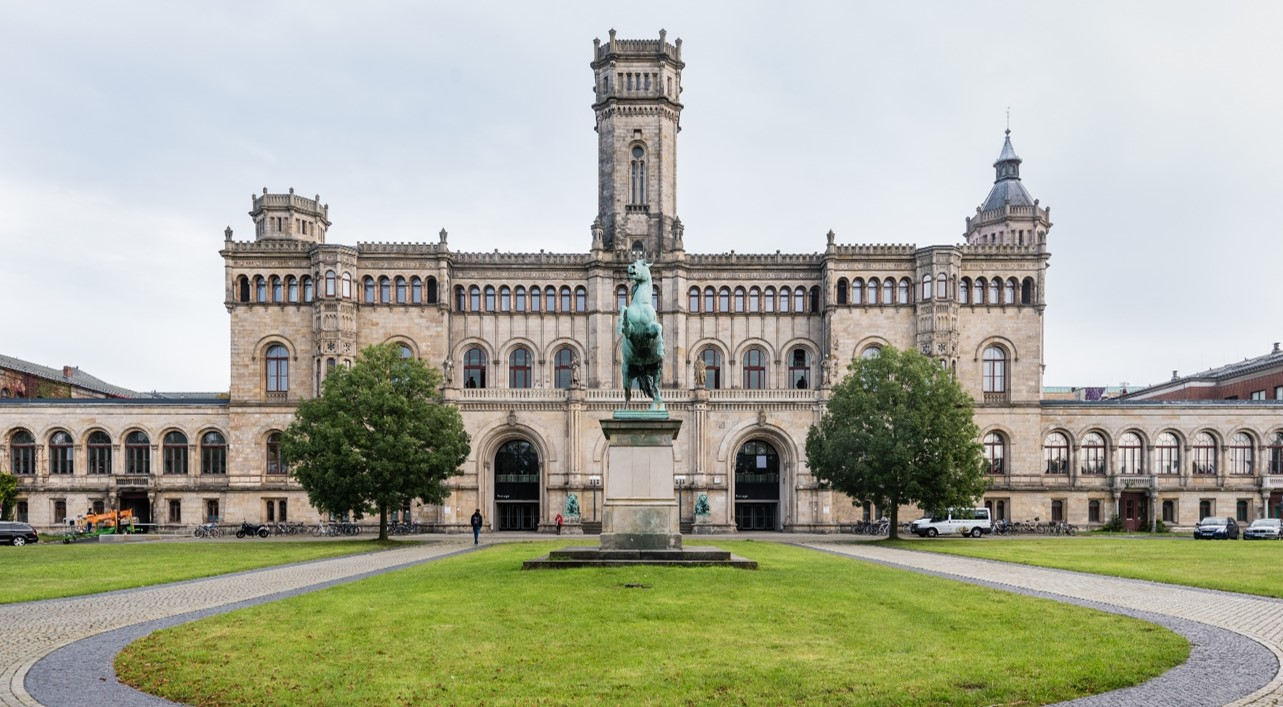
\includegraphics[width=0.65\textwidth]{figures/luh_default_presentation_title_image.jpg}}

% Title page: luhstyle
% \setbeamertemplate{title page}[luhstyle]
% % Add optional title image here
% \addtitlepageimage{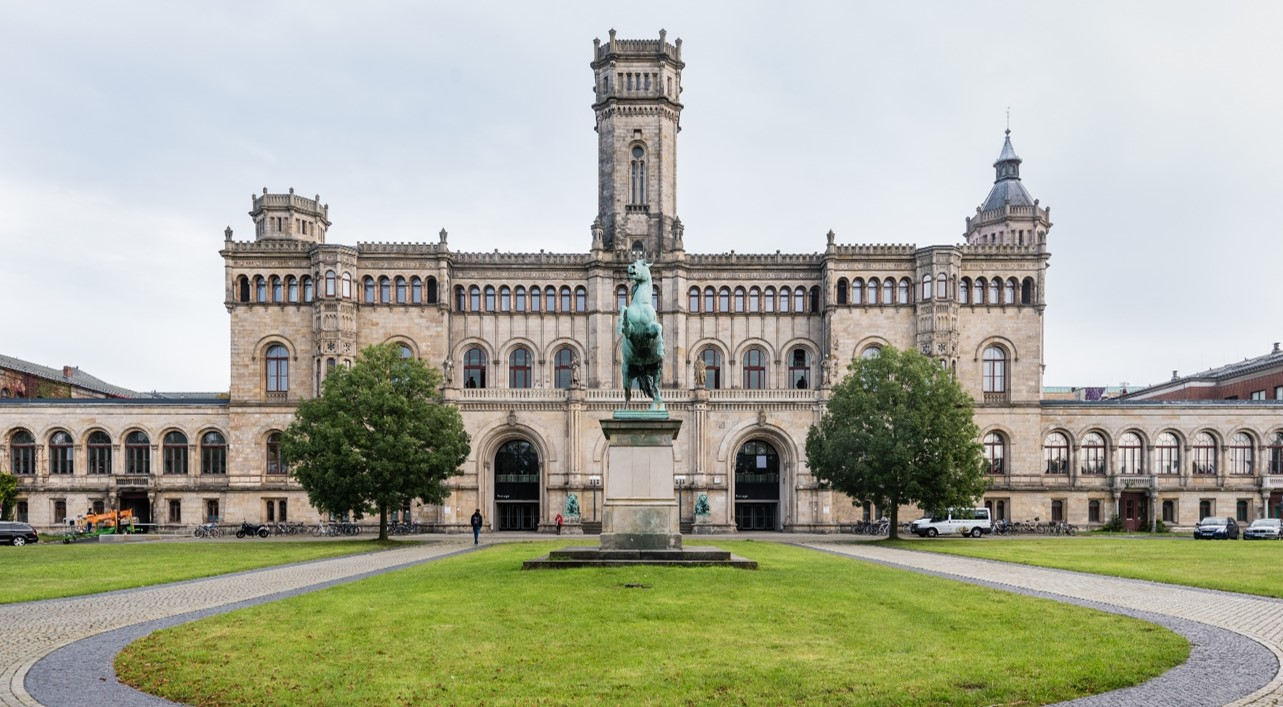
\includegraphics[width=0.75\textwidth]{figures/luh_default_presentation_title_image.jpg}}

\author[Abedjan \& Lindauer]{Ziawasch Abedjan \& Marius Lindauer\\[1em]
	
\includegraphics[height=\logoheight]{../latex_main/figures/luh_logo_rgb_0_80_155.pdf}\qquad
	
\includegraphics[height=\logoheight]{../latex_main/figures/DBIS_Kurzlogo.png}\qquad

\includegraphics[height=\logoheight]{../latex_main/figures/TNT_darkv4}\qquad

\includegraphics[height=\logoheight]{../latex_main/figures/L3S.jpg}	}
\date{Summer Term 2022; \hspace{0.5em} {
\includegraphics[height=1.5em]{../latex_main/figures/Cc-by-nc-sa_icon.svg.png}}; based on \href{https://ds100.org/fa21/}{[DS100]}
}


%%% Custom Packages
%----------------------------------------------------------------------
% Create dummy content
\usepackage{blindtext}

% Adds a frame with the current page layout. Just call \layout inside of a frame.
\usepackage{layout}


%%% Macros
%\renewcommand{\vec}[1]{\mathbf{#1}}
% \usepackage{bm}
%\let\vecb\bm

\title[Introduction]{DS: Clustering, Part 1}
\subtitle{Picking K}

\graphicspath{ {./figure/} }
%\institute{}


\begin{document}
	
	\maketitle
	\begin{frame}{Picking K}
	    The algorithms we’ve discussed today require us to pick a K before we start
	    \begin{columns}
	        \begin{column}{.6\textwidth}
	                \begin{itemize}
	                    \item But how do we pick K?
	                \end{itemize}
	                \begin{figure}
	                    \centering
	                    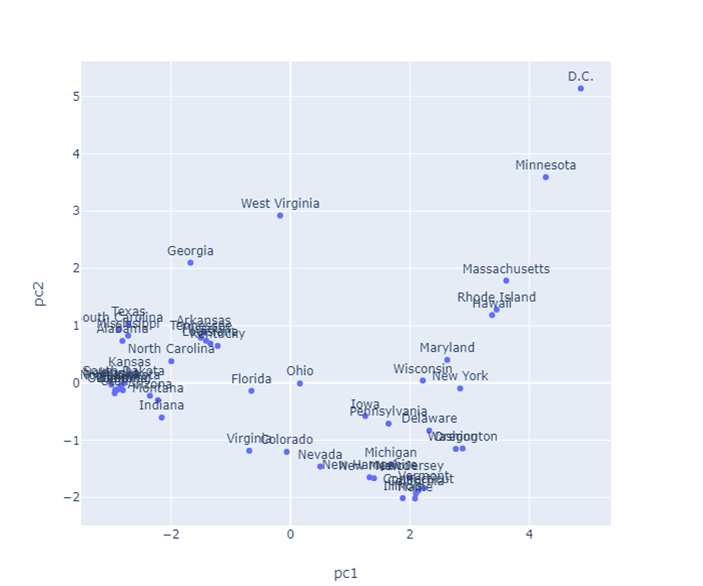
\includegraphics[scale=.45]{Bild55}
	                \end{figure}
	        \end{column}
	        
	        
	        \begin{column}{.4\textwidth}
	        \\
	        \bigskip
	            Often, best K is subjective
	                \begin{itemize}
	                    \item Example: State plot that you will see in HW12
	                    \item How many clusters are there here?
	                \end{itemize}
	        \end{column}
	    \end{columns}
	\end{frame}
	
	
	\begin{frame}{Picking K: Elbow Method}
	    For K-Means, one approach is to plot inertia versus many different K values
	    \begin{itemize}
	        \item Pick the K in the “elbow”, where we get diminishing returns afterwards
	        \item Note: Big complicated data often lacks an elbow
	    \end{itemize}
	    \begin{figure}
	        \centering
	        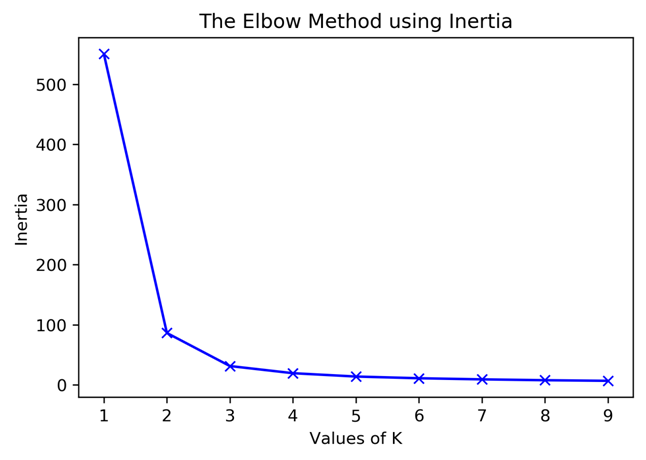
\includegraphics[scale=.65]{Bild56}
	    \end{figure}
	\end{frame}
	
	
	
	\begin{frame}{Silhouette Scores}
	    To evaluate how “well clustered” a specific data point is, we can use the silhouette score, a.k.a. the “silhouette width” 
	    \begin{itemize}
	        \item High score: Near the other points in its X’s cluster
	        \item Low score: Far from the other points in its cluster
	    \end{itemize}
	    \begin{columns}
	        \begin{column}{.5\textwidth}
	                \begin{figure}
	                    \centering
	                    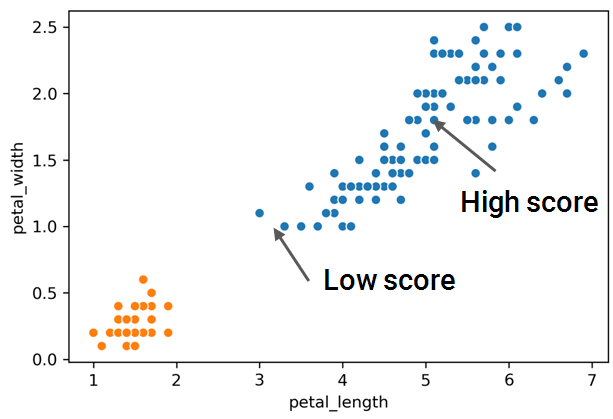
\includegraphics[scale=.35]{Bild57}
	                \end{figure}
	        \end{column}
	        
	        
	        \begin{column}{.5\textwidth}
	                For a data point X, score S is:
	                \begin{itemize}
	                    \item A = avg distance to other points in cluster
	                    \item B = avg distance to points in closest cluster
	                    \item S = (B - A) / max(A, B)
	                \end{itemize}
	        \end{column}
	        
	        
	    \end{columns}
	\end{frame}
	
	
	
	\begin{frame}{Silhouette Scores}
	    For a data point X:
	    \begin{itemize}
	        \item A = average distance to other points in X’s cluster 
	        \item B = average distance to points in closest cluster
	        \item S = (B - A) / max(A, B)
	    \end{itemize}
	    \begin{columns}
	        \begin{column}{.5\textwidth}
	                \begin{figure}
	                    \centering
	                    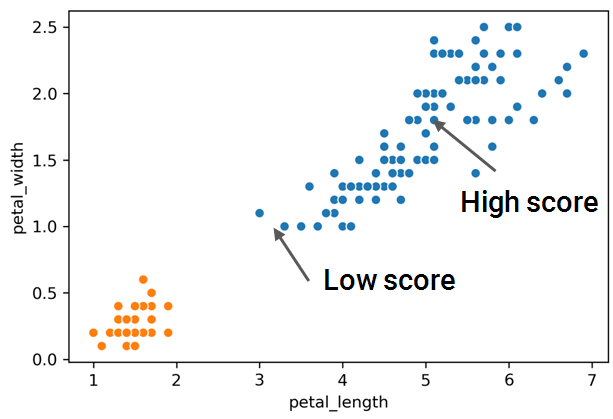
\includegraphics[scale=.35]{Bild57}
	                \end{figure}
	        \end{column}
	        
	        
	        \begin{column}{.5\textwidth}
	                What is the highest possible S?
	                \begin{itemize}
	                    \item How can this happen?
	                \end{itemize}
	                \pause
	                Highest possible S is 1
	                \begin{itemize}
	                    \item This happens if every point in X’s cluster is right on top of X
	                \end{itemize}
	        \end{column}
	        
	        
	    \end{columns}
	\end{frame}
	
	
	
	\begin{frame}{Silhouette Scores}
	    For a data point X:
	    \begin{itemize}
	        \item A = average distance to other points in X’s cluster 
	        \item B = average distance to points in closest cluster
	        \item S = (B - A) / max(A, B)
	    \end{itemize}
	    \begin{columns}
	        \begin{column}{.5\textwidth}
	                \begin{figure}
	                    \centering
	                    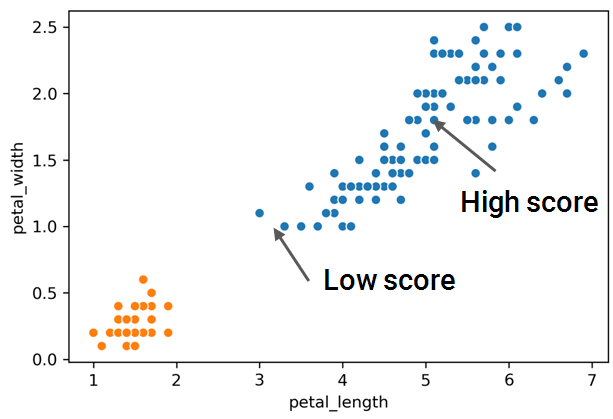
\includegraphics[scale=.35]{Bild57}
	                \end{figure}
	        \end{column}
	        
	        
	        \begin{column}{.5\textwidth}
	               Can S be negative?
	               \pause
	               \begin{itemize}
	                   \item Yes. Average distance to X’s clustermates is larger than distance to the closest cluster
	                   \pause
	                   \item Example: The “low score” point on the right has  S = -0.13
	               \end{itemize}
	        \end{column}
	        
	        
	    \end{columns}
	\end{frame}
	
	
	
	
	\begin{frame}{Silhouette Scores}
	    We can plot the Silhouette Scores for all of our data points
	    \begin{itemize}
	        \item Points with large silhouette widths are deeply embedded in their cluster
	        \item Red dotted line shows the average
	    \end{itemize}
	    \begin{columns}
	        \begin{column}{.5\textwidth}
	                \begin{figure}
	                    \centering
	                    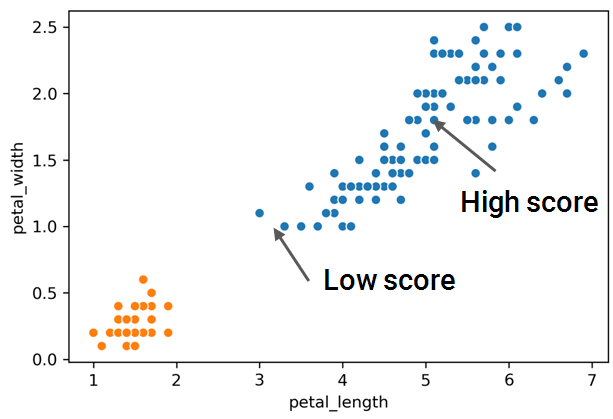
\includegraphics[scale=.35]{Bild57}
	                \end{figure}
	        \end{column}
	        
	        
	        \begin{column}{.5\textwidth}
	               \begin{figure}
	                    \centering
	                    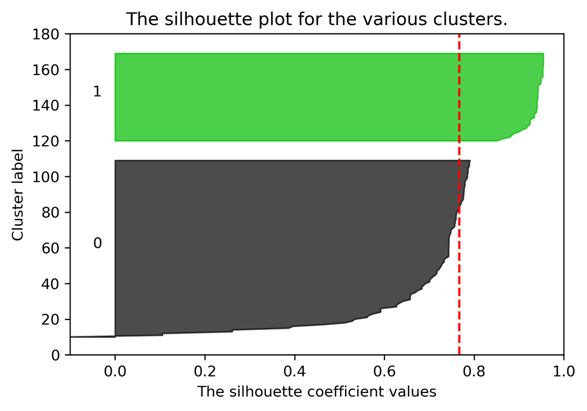
\includegraphics[scale=.65]{Bild58}
	                \end{figure}
	        \end{column}
	        
	        
	    \end{columns}
	\end{frame}
	
	
	\begin{frame}{Silhouette Scores, K = 2 vs. K = 3}
	    \begin{figure}
	        \centering
	        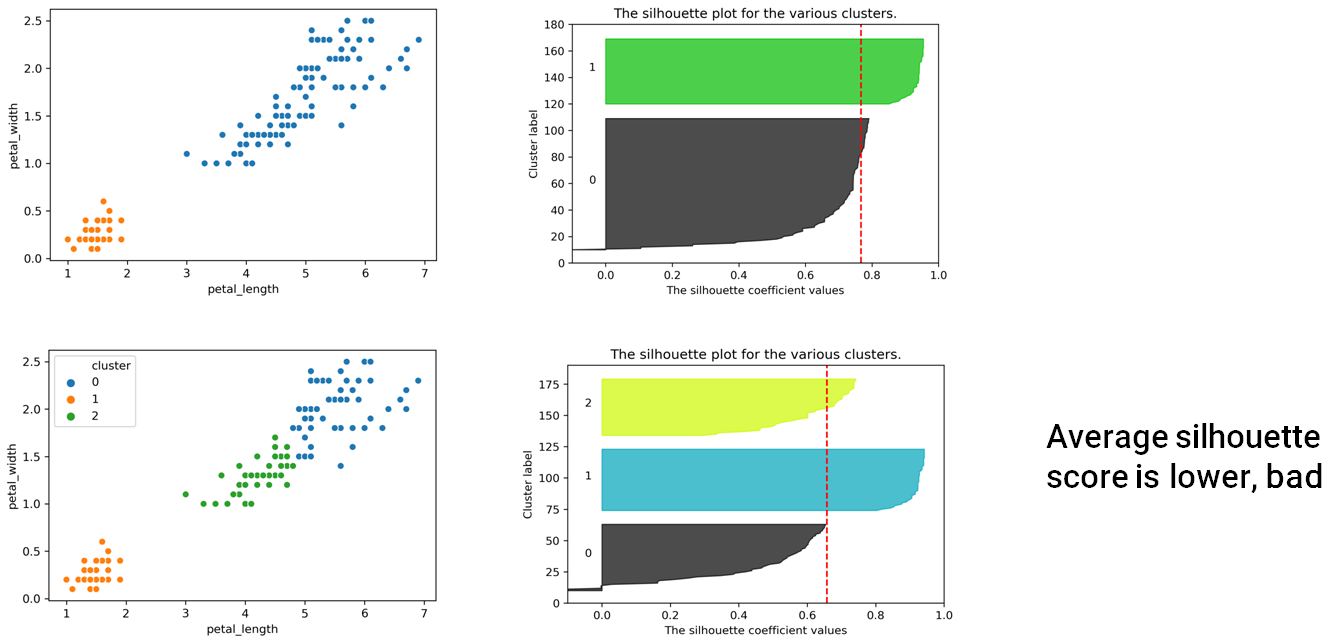
\includegraphics[scale=.35]{Bild59}
	    \end{figure}
	\end{frame}
	
	
	\begin{frame}{Picking K: Real World Metrics (Example via Andrew Ng)}
	    Sometimes you can rely on real world metrics to guide your choice of K\\
	    \bigskip
	    Perform 2 clusterings:
	    \begin{itemize}
	        \item Cluster heights and weights of customers with K = 3 to design Small, Medium, and Large shirts
	        \item Cluster heights and weights of customers with K = 5 to design XS, S, M, L, and XL shirts
	    \end{itemize}
	    \bigskip
	    To pick K:
	    \begin{itemize}
	        \item Consider projected costs and sales for the 2 different Ks
	        \item Pick the one that maximizes profit
	    \end{itemize}
	\end{frame}
	
	
	\begin{frame}{Summary}
	    Today we discussed a new machine learning goal: Clustering\\
	    \bigskip
	    Saw two solutions:
	    \begin{itemize}
	        \item K-Means
	        \begin{itemize}
	            \item Tries to optimize a loss function called inertia -- no known algorithm to do this optimally
	        \end{itemize}
	        \item Agglomerative
	    \end{itemize}
	    \bigskip
	    Our version of these algorithms required a hyperparameter k
	    \begin{itemize}
	        \item 4 ways to pick K: Intuitively, Elbow method, Silhouette scores, Harnessing real world metrics
	    \end{itemize}
	\end{frame}
	
	
	
	\begin{frame}{Bigger Picture Summary}
	    There are many Machine Learning problems
	    \begin{itemize}
	        \item Each can be addressed by many different solution techniques
	        \item Each has many metrics for evaluating success / loss
	    \end{itemize}
	    \bigskip
	    Many solution technique can be used for multiple problem types
	    \begin{itemize}
	        \item Example: Linear models can be used for regression and classification
	    \end{itemize}
	    \bigskip
	    We’ve only scratched the surface. Haven’t discussed many important ideas
        \begin{itemize}
            \item One hugely important solution technique: Neural Networks / Deep Learning
            \begin{itemize}
                \item See other courses in CS and Data Science for more
            \end{itemize}
            \item Will provide some specific course recommendations in the last lecture
        \end{itemize}
	\end{frame}
	
	
	
	\begin{frame}{Review: Taxonomy of Machine Learning}
	    \begin{figure}
	        \centering
	        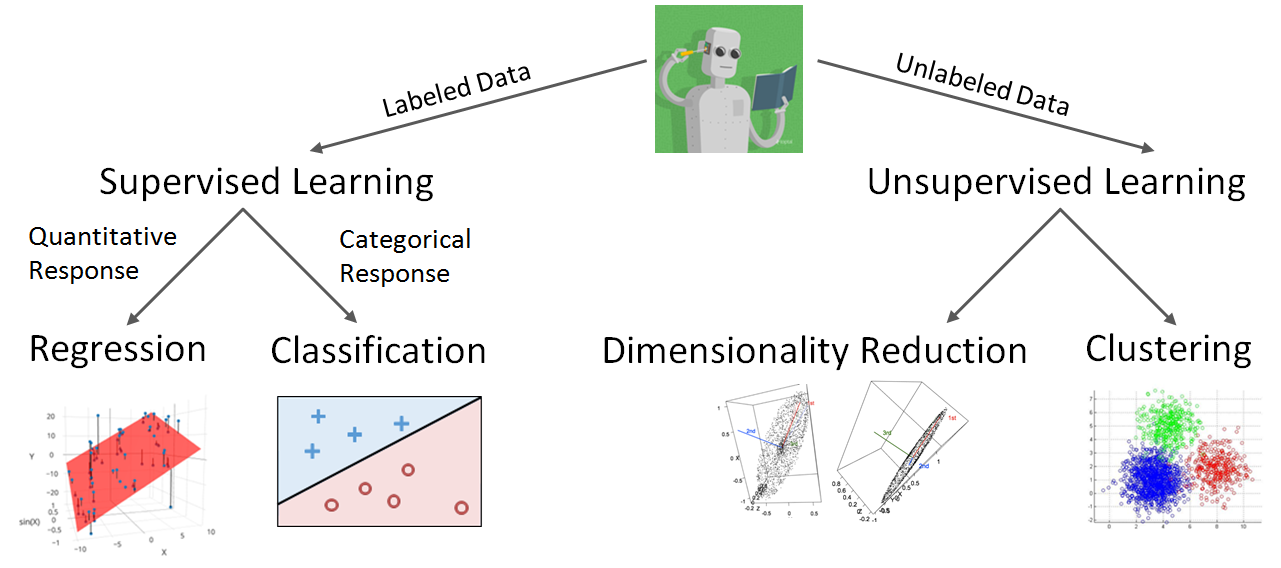
\includegraphics[scale=.4]{Bild60}
	    \end{figure}
	\end{frame}
\end{document}